\begin{figure}[ht]
\centering
\vspace{-6mm}
\centerline{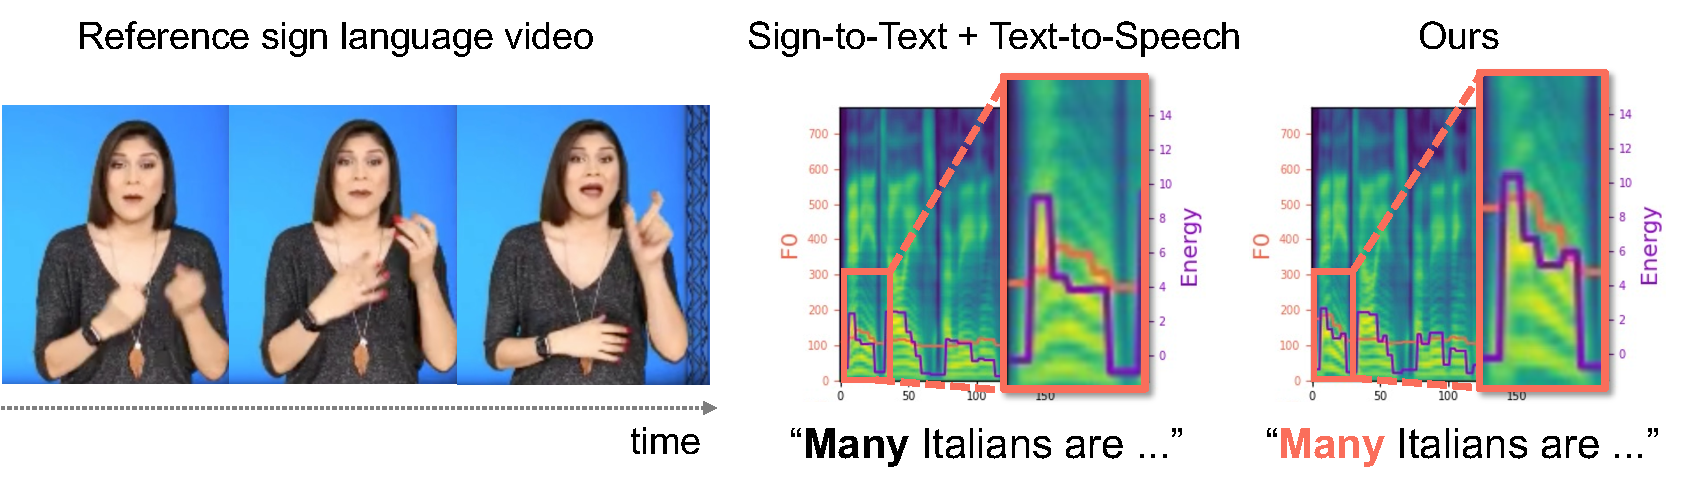
\includegraphics[width=\linewidth]{assets/heading.pdf}}
\vspace{-5mm}
\caption{
% We propose S2PFormer for \emph{Sign-to-Speech Prosody Transfer} task. 
% Our key idea is to directly transfer the sign language prosody into speech synthesis by ensuring that the prosodic cues of the sign language can be reconstructed from the synthesized speech.
In the reference sign language video (left), the first phrase, ``many Italians,'' is emphasized through rapid hand movements and facial expressions. The two-stage baseline (middle) fails to reflect this prosody, whereas our approach (right) successfully captures the emphasis on ``many.''}
\vspace{-8mm}
\label{fig:pipeline}
\end{figure}

\begin{abstract}
Sign language is a vital means of communication for individuals with hearing impairments.
Deep learning models have improved sign-to-text translation and made it easier for non-signers to understand signed messages.
However, sign language also carries non-textual information that these systems often miss.
Existing 2-stage pipelines (sign-to-text followed by text-to-speech) rely solely on textual intermediaries,
which inevitably strip away much of the prosodic detail conveyed by the signer's movements.
To address this issue, we propose a novel, \emph{Sign-to-Speech \shibata{Global} Prosody Transfer},
aimed at capturing the \manabe {global} prosodic nuances conveyed by sign language 
and integrating them directly into synthesized speech.
This task is extremely challenging for three main reasons.
First, sign language translation is a specialized, complex task, and high-quality datasets that pair sign language with speech are unavailable.
Second, speech prosody itself is intricate, thereby adding another layer of complexity to the translation process.
Finally, the relationship between sign language prosody and spoken prosody is highly subtle, and no established method currently exists for mapping them directly.
To overcome these challenges, we introduce the S2PFormer (Sign-to-Prosody Transformer).
Our model leverages sign language prosody reconstruction to enable training on unpaired datasets without direct correspondence between sign language and speech.
In addition, by applying cross-attention to human joint movements and textual information, the model can capture subtle prosodic signals.
Extensive experiments demonstrate that the proposed method can synthesize speech that faithfully reflects the emotional content of sign language, thereby opening new possibilities for more natural sign language communication. Our code will be available upon acceptance.

\keywords{First keyword  \and Second keyword \and Another keyword.}
\end{abstract}
